\documentclass[spanish,letterpaper,oneside]{article}

% Datos del documento
\def\documenttitle {El futuro del aprendizaje en el siglo XXI}
\def\documentsubtitle {Reporte de lectura y mapa conceptual}
\def\documentsubject {Actividad 1}
\def\documentauthor {Mtro. Martin Jonathan de la Cruz Munoz}
\def\coursename {Fundamentos para la enseñanza y el aprendizaje I}
\def\coursecode {MAEM}

% Identidad institucional
\def\universityname {Instituto de Investigación, Innovación y Estudios de Posgrado para la Educación del Estado de Nuevo León}
\def\universityfaculty {Maestría en Aprendizaje y Enseñanza de las Matemáticas}
\def\universitydepartment {Fundamentos para la enseñanza y el aprendizaje I}
\def\universitydepartmentimage {img/iiiepe/marca-iiiepe.png}
\def\universitydepartmentimagecfg {height=1.75cm}
\def\universitylocation {Monterrey, Nuevo León}
\def\studentfullname {Mtro. Martin Jonathan de la Cruz Muñoz}
\def\studentid {00874}
\def\studentemail {martin.delacruz@campus.iiiepe.edu.mx}
\def\programperiod {1er tetramestre, marzo--julio de 2026}
\def\programmodality {Modalidad presencial}
\def\programshort {MAEM}

\def\authortable {
  \begin{tabular}{ll}
    \textbf{Alumno:} & \studentfullname \\
    Matrícula: & \studentid \\
    Correo institucional: & \studentemail \\
    \textit{Figura docente:} & No especificada \\
    Unidad: & \coursename \\
    Programa: & \programshort \\
    Periodo: & \programperiod \\
    & \\
    \multicolumn{2}{l}{Fecha de realización: \today} \\
    \multicolumn{2}{l}{\universitylocation}
  \end{tabular}
}

\input{template}

\usepackage{helvet}
\renewcommand{\familydefault}{\sfdefault}
\usepackage{array}
\usepackage{longtable}
\usepackage{pdflscape}
\usepackage{tikz}
\usetikzlibrary{arrows.meta,positioning,calc,fit,backgrounds}

\definecolor{iiiepeNavy}{HTML}{163B5C}
\definecolor{iiiepeBlue}{HTML}{1F6F9F}
\definecolor{iiiepeAqua}{HTML}{20B7A8}
\definecolor{iiiepeOrange}{HTML}{F28C28}
\definecolor{iiiepePaper}{HTML}{F6F8F7}
\definecolor{iiiepeInk}{HTML}{1E2A32}
\def\portraittitlecolor {iiiepeNavy}
\setcitestyle{authoryear,open={(},close={)}}

% Marca de agua de portada
\newcommand{\insertcoverwatermark}{%
  \AddToShipoutPictureBG*{%
    \begin{tikzpicture}[remember picture,overlay]
      \node[opacity=.09,inner sep=0pt] at (current page.center)
      {
\includegraphics[width=.58\paperwidth]{img/iiiepe/logo-puntos.png}};
    \end{tikzpicture}%
  }%
}

\begin{document}

\insertcoverwatermark
\templatePortrait
\templatePagecfg
\onehalfspacing

\begin{abstractd}
Este reporte analiza la tesis central de Cynthia Luna Scott: el contenido, la pedagogía y la evaluación deben transformarse porque la escuela heredada de la era industrial ya no prepara suficientemente para un mundo complejo, digital e interdependiente. Mediante lectura analítica y la técnica de mapa conceptual se organizan las fuerzas del cambio, las insuficiencias del modelo vigente y las orientaciones de la reforma. Se sostiene que innovar no equivale a añadir tecnología, sino a rediseñar experiencias para que el estudiantado investigue, colabore, argumente, resuelva problemas y autorregule su aprendizaje. La aportación del texto permanece vigente, aunque sus datos tecnológicos de 2014 deben leerse como evidencia histórica y no como descripción del presente.
\end{abstractd}

\templateIndex
\templateFinalcfg

\section{Introducción}

La discusión sobre el futuro del aprendizaje no se reduce a anticipar dispositivos o profesiones. Su problema de fondo es la distancia entre una escuela organizada para transmitir contenidos estables y una realidad caracterizada por incertidumbre, interdependencia, aceleración tecnológica y problemas que desbordan una sola disciplina. En \textit{El futuro del aprendizaje 1}, Scott examina por qué esa distancia obliga a revisar tanto lo que se aprende como la manera de aprenderlo \citep{scott2015futuro}.

El propósito de este reporte es reconstruir el argumento de la autora, distinguir sus principales fuerzas explicativas y valorar sus implicaciones para la enseñanza de las matemáticas. Como producto de síntesis se presenta un mapa conceptual elaborado conforme a la técnica 81 del repertorio de la Universidad Abierta y a Distancia de México: conceptos jerarquizados, palabras de enlace y relaciones cruzadas que permiten leer proposiciones completas \citep{lopez2022mapa,unadm2023tecnicas}.

La postura que guía el análisis es que la reforma educativa no debe comenzar por la herramienta, sino por el tipo de actividad intelectual y social que se desea producir. La tecnología puede ampliar la participación, la personalización y el acceso; sin embargo, solo genera valor educativo cuando se articula con propósitos formativos, mediación docente y evaluación congruente.

\section{Ficha de la lectura}

\begin{longtable}{@{}p{0.23\linewidth}p{0.70\linewidth}@{}}
\toprule
\textbf{Elemento} & \textbf{Descripción} \\
\midrule
Autoría & Cynthia Luna Scott. \\
Título & \textit{El futuro del aprendizaje 1: ¿Por qué deben cambiar el contenido y los métodos de aprendizaje en el siglo XXI?} \\
Publicación & UNESCO, serie \textit{Investigación y prospectiva en educación: contribuciones temáticas}, núm. 13. \\
Año y documento & 2015; ED-2015/WS/22. \\
Tipo de texto & Documento de trabajo y revisión amplia de literatura sobre prospectiva educativa. \\
Pregunta central & ¿Qué transformaciones sociales, laborales, tecnológicas y educativas justifican reformar el contenido y los métodos de aprendizaje? \\
Tesis reconstruida & La escuela debe desplazarse de la transmisión uniforme hacia aprendizajes autónomos, colaborativos, personalizados y vinculados con problemas reales, sin renunciar a una visión humanística de la educación. \\
\bottomrule
\end{longtable}

\section{Reporte de lectura}

\subsection{Propósito y organización argumentativa}

Scott presenta el primero de tres estudios sobre el aprendizaje del siglo XXI. Este volumen no ofrece todavía un catálogo definitivo de competencias ni una metodología única; construye el diagnóstico que vuelve necesaria la transformación. Su razonamiento sigue una secuencia reconocible: identifica cambios del entorno, muestra el desfase de la institución escolar, examina las características y expectativas de quienes aprenden, incorpora las demandas del trabajo y la ciudadanía, y concluye con la necesidad de modificar currículo, pedagogía y evaluación \citep{scott2015futuro}.

Este alcance es importante porque evita leer el documento como una receta. La autora integra estudios prospectivos y reportes internacionales para sostener una dirección de cambio. Por ello, el valor principal del texto reside en relacionar presiones que suelen analizarse por separado: abandono escolar, desmotivación, transformación laboral, digitalización, movilidad humana, crisis ambientales y participación cívica.

\subsection{De la transmisión a la formación para la complejidad}

La primera idea central es que preparar para el siglo XXI exige más que acumular información. La mundialización, los cambios demográficos, la incertidumbre laboral y los problemas socioambientales requieren pensamiento crítico, creatividad, comunicación, colaboración y capacidad para resolver situaciones sin una respuesta evidente. La alfabetización básica sigue siendo indispensable, pero deja de ser suficiente cuando las personas deben interpretar información contradictoria, aprender durante toda la vida y actuar con otros en contextos diversos \citep{scott2015futuro}.

La lectura recupera una visión integral de la educación. Los fines económicos y laborales no agotan su sentido: también importa formar ciudadanía capaz de comprender asuntos públicos, deliberar con evidencia y participar responsablemente. Esta orientación coincide con la tradición humanística que concibe aprender como aprender a conocer, hacer, convivir y ser \citep{delors1996educacion}. Así, una reforma pertinente debe equilibrar empleabilidad, desarrollo personal, justicia social y sostenibilidad.

\subsection{Fuerzas que impulsan el cambio}

El texto reúne cuatro conjuntos de presiones. Primero, un mundo interconectado produce problemas complejos que demandan perspectivas interdisciplinarias y cooperación intercultural. Segundo, el estudiantado participa en ecosistemas digitales, espera mayor capacidad de elección y aprende también fuera de la escuela. Tercero, el desinterés y el abandono revelan que una parte de la oferta educativa no logra construir pertinencia. Cuarto, el trabajo cambia con rapidez y demanda aprender, desaprender y actualizar competencias de manera continua \citep{scott2015futuro}.

Estas fuerzas no operan de modo aislado. La expansión tecnológica modifica la circulación de información y el trabajo; esas transformaciones cambian las expectativas del alumnado; cuando la escuela mantiene actividades descontextualizadas, aumenta la percepción de irrelevancia. La consecuencia no es que toda práctica anterior deba desecharse, sino que cada contenido y método necesita justificarse por su contribución a una formación transferible.

\subsection{Transformación del papel docente y de la experiencia escolar}

Scott prevé instituciones centradas menos en la enseñanza como exposición y más en el aprendizaje como actividad del estudiante. En ese marco, el profesorado deja de ser únicamente fuente de respuestas y asume funciones de diseño, mediación, acompañamiento y retroalimentación. El aprendizaje se vuelve más personal, participativo, práctico y colectivo; puede ocurrir en distintos tiempos y espacios y apoyarse en redes y recursos digitales \citep{scott2015futuro}.

Este desplazamiento no disminuye la relevancia docente. Por el contrario, la incrementa: cuando la información es abundante, se necesita criterio para seleccionar fuentes, formular problemas, secuenciar retos y convertir la actividad en comprensión. La mediación también debe cuidar inclusión y equidad, pues el acceso a dispositivos no garantiza conectividad, alfabetización informacional ni condiciones equivalentes de participación.

\subsection{Tecnología: medio y no finalidad}

Uno de los aportes más útiles de la lectura es evitar el determinismo tecnológico. El documento reconoce la potencia de Internet, las redes y los dispositivos móviles, pero advierte que incorporarlos como accesorios no transforma la pedagogía. Su valor surge cuando hacen posibles comunicación, creación, colaboración, acceso flexible y producción de conocimiento que no podrían alcanzarse del mismo modo con una clase exclusivamente transmisiva \citep{scott2015futuro}.

Los datos de penetración tecnológica incluidos en el anexo corresponden a 2014. Por tanto, sirven para comprender el momento histórico del argumento, pero no deben emplearse como estadísticas actuales. Esta precaución fortalece la lectura crítica: el diagnóstico estructural puede conservar vigencia aunque algunos indicadores y ejemplos de plataforma hayan envejecido.

\subsection{Implicaciones para currículo y evaluación}

Si el propósito cambia de reproducir información a movilizar saberes, también debe cambiar la evaluación. No es coherente declarar como objetivos la colaboración, la creatividad o la resolución de problemas y medir únicamente recuerdo individual de datos. Se requieren desempeños observables: investigaciones, modelos, explicaciones, proyectos, debates, soluciones justificadas y procesos de revisión.

El currículo, en consecuencia, debe seleccionar menos contenidos aislados y construir conexiones más profundas. La personalización no implica eliminar objetivos comunes, sino ofrecer rutas, apoyos y formas de participación que reconozcan diferencias. Desde una perspectiva de bien común, la innovación necesita mantener la responsabilidad pública, la inclusión y el sentido humanístico de la educación \citep{unesco2015replantear}.

\section{Mapa conceptual}

La técnica del mapa conceptual es pertinente como control de lectura porque obliga a seleccionar conceptos, jerarquizarlos y convertir sus vínculos en proposiciones. El mapa siguiente responde a la pregunta: \textit{¿por qué y hacia dónde debe transformarse el aprendizaje del siglo XXI?} No reproduce el índice de la lectura; reconstruye su lógica causal y agrega relaciones transversales para mostrar que entorno, escuela, actores y reforma forman un sistema \citep{lopez2022mapa}.

\clearpage
\pagestyle{empty}
\begin{landscape}
\begin{figure}[p]
\centering
\resizebox{0.96\linewidth}{!}{%
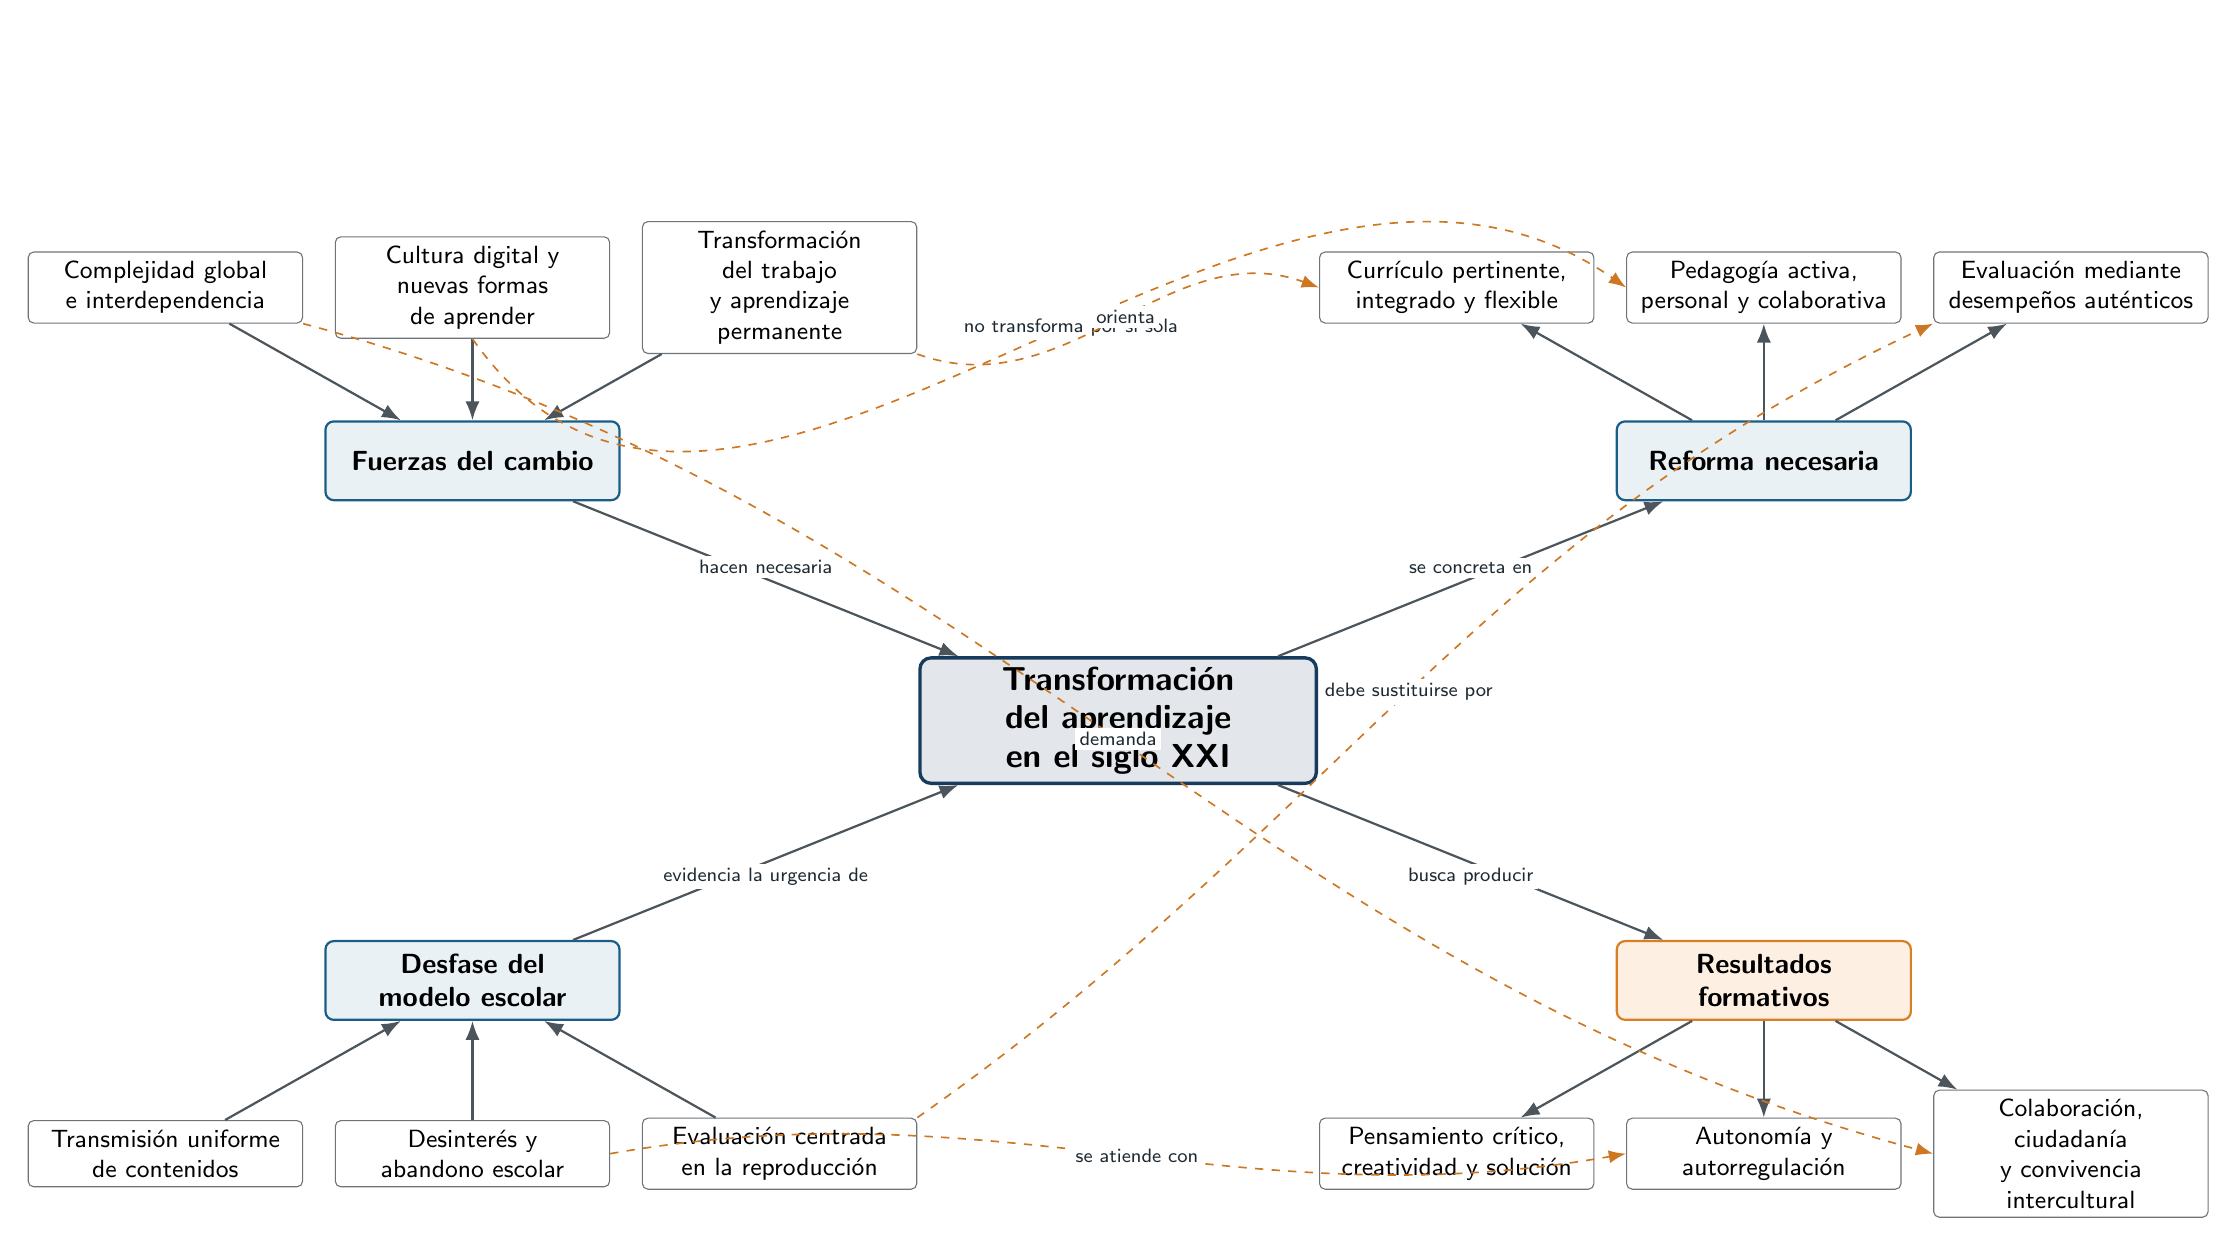
\begin{tikzpicture}[
  font=\sffamily,
  root/.style={rounded corners=4pt,draw=iiiepeNavy,very thick,fill=iiiepeNavy!12,text width=4.8cm,align=center,minimum height=1.25cm,font=\bfseries\large},
  branch/.style={rounded corners=3pt,draw=iiiepeBlue!85!black,thick,fill=iiiepeBlue!10,text width=3.5cm,align=center,minimum height=1cm,font=\bfseries},
  leaf/.style={rounded corners=2pt,draw=iiiepeInk!65,fill=white,text width=3.25cm,align=center,minimum height=.82cm,font=\small},
  outcome/.style={rounded corners=3pt,draw=iiiepeOrange!90!black,thick,fill=iiiepeOrange!13,text width=3.5cm,align=center,minimum height=1cm,font=\bfseries},
  edge/.style={-{Latex[length=2.4mm]},thick,draw=iiiepeInk!80},
  cross/.style={-{Latex[length=2.2mm]},semithick,dashed,draw=iiiepeOrange!85!black},
  label/.style={fill=white,inner sep=1.5pt,font=\scriptsize,text=iiiepeInk}
]
\node[root] (center) at (0,0) {Transformación del aprendizaje\\en el siglo XXI};

\node[branch] (forces) at (-8.2,3.3) {Fuerzas del cambio};
\node[leaf] (complex) at (-12.1,5.5) {Complejidad global\\e interdependencia};
\node[leaf] (digital) at (-8.2,5.5) {Cultura digital y\\nuevas formas de aprender};
\node[leaf] (work) at (-4.3,5.5) {Transformación del trabajo\\y aprendizaje permanente};

\node[branch] (gap) at (-8.2,-3.3) {Desfase del modelo escolar};
\node[leaf] (transmission) at (-12.1,-5.5) {Transmisión uniforme\\de contenidos};
\node[leaf] (disengage) at (-8.2,-5.5) {Desinterés y\\abandono escolar};
\node[leaf] (assessment) at (-4.3,-5.5) {Evaluación centrada\\en la reproducción};

\node[branch] (reform) at (8.2,3.3) {Reforma necesaria};
\node[leaf] (curriculum) at (4.3,5.5) {Currículo pertinente,\\integrado y flexible};
\node[leaf] (pedagogy) at (8.2,5.5) {Pedagogía activa,\\personal y colaborativa};
\node[leaf] (evidence) at (12.1,5.5) {Evaluación mediante\\desempeños auténticos};

\node[outcome] (purposes) at (8.2,-3.3) {Resultados formativos};
\node[leaf] (skills) at (4.3,-5.5) {Pensamiento crítico,\\creatividad y solución};
\node[leaf] (agency) at (8.2,-5.5) {Autonomía y\\autorregulación};
\node[leaf] (citizenship) at (12.1,-5.5) {Colaboración, ciudadanía\\y convivencia intercultural};

\draw[edge] (forces) -- node[label,above]{hacen necesaria} (center);
\draw[edge] (gap) -- node[label,below]{evidencia la urgencia de} (center);
\draw[edge] (center) -- node[label,above]{se concreta en} (reform);
\draw[edge] (center) -- node[label,below]{busca producir} (purposes);

\foreach \n in {complex,digital,work} {\draw[edge] (\n) -- (forces);}
\foreach \n in {transmission,disengage,assessment} {\draw[edge] (\n) -- (gap);}
\foreach \n in {curriculum,pedagogy,evidence} {\draw[edge] (reform) -- (\n);}
\foreach \n in {skills,agency,citizenship} {\draw[edge] (purposes) -- (\n);}

\draw[cross] (digital.south) to[out=-55,in=145] node[label,pos=.55]{no transforma por sí sola} (pedagogy.west);
\draw[cross] (work.south east) to[out=-20,in=160] node[label,pos=.52]{orienta} (curriculum.west);
\draw[cross] (assessment.north east) to[out=35,in=205] node[label,pos=.50]{debe sustituirse por} (evidence.south west);
\draw[cross] (disengage.east) to[out=10,in=190] node[label,pos=.52]{se atiende con} (agency.west);
\draw[cross] (complex.south east) to[out=-15,in=165] node[label,pos=.50]{demanda} (citizenship.west);
\end{tikzpicture}%
}
\caption{Mapa conceptual del argumento de \citet{scott2015futuro}. Elaboración propia con base en la técnica 81 de \citet{lopez2022mapa}.}
\label{fig:mapa-futuro-aprendizaje}
\end{figure}
\end{landscape}
\pagestyle{fancy}
\clearpage

\subsection{Lectura del mapa}

El concepto central se explica por dos entradas diagnósticas y dos salidas propositivas. Las fuerzas del cambio hacen necesaria la transformación, mientras el desfase escolar muestra por qué es urgente. La transformación se concreta en una reforma articulada de currículo, pedagogía y evaluación, cuyo resultado esperado es una formación que combine agencia individual y responsabilidad colectiva.

Las relaciones cruzadas expresan cuatro criterios. La tecnología no transforma por sí sola la pedagogía; la evolución del trabajo orienta, pero no debe monopolizar, el currículo; una evaluación reproductiva debe reemplazarse por evidencias auténticas; y la pertinencia de las experiencias puede contribuir a atender el desinterés. De este modo, el mapa evita convertir la lectura en una lista y hace visible su estructura de causas, decisiones y consecuencias.

\section{Valoración crítica y aplicación a la enseñanza de las matemáticas}

La principal fortaleza del documento es su mirada sistémica. Scott no atribuye el cambio a una moda, sino a la convergencia de presiones sociales, tecnológicas, económicas y cívicas. También acierta al vincular el contenido con el método: enseñar nuevas competencias mediante prácticas centradas exclusivamente en exposición y repetición produciría una contradicción entre fines y medios.

Su límite procede del género prospectivo y de la fecha de publicación. Algunas previsiones se apoyan en informes y datos de uso tecnológico que hoy requieren actualización. Además, hablar de ``el estudiante del siglo XXI'' puede ocultar desigualdades de acceso, contexto, edad y experiencia. No todo alumnado posee la misma autonomía digital ni toda innovación es transferible sin adaptación local. Por ello, sus orientaciones deben convertirse en hipótesis de diseño que se prueban con evidencia, no en mandatos universales.

En matemáticas, esta lectura conduce a reemplazar parte de la ejercitación descontextualizada por problemas abiertos que exijan modelar, representar, argumentar y comparar estrategias. Por ejemplo, ante un fenómeno de consumo de agua, movilidad o propagación, el grupo puede definir variables, seleccionar datos, construir un modelo, discutir supuestos y comunicar límites. La tecnología serviría para explorar representaciones o contrastar escenarios, pero la evidencia de aprendizaje estaría en la calidad de las decisiones y justificaciones.

La evaluación congruente integraría productos y proceso: formulación del problema, elección de herramientas, precisión matemática, explicación, colaboración, revisión y transferencia. El docente diseñaría andamiajes y preguntas, observaría estrategias y ofrecería retroalimentación. Así, la autonomía no significaría abandono, sino responsabilidad progresiva dentro de una estructura deliberada.

\section{Conclusión}

La lectura permite concluir que el futuro del aprendizaje es, ante todo, una decisión pedagógica y social. Las transformaciones del entorno muestran la insuficiencia de una escuela dedicada únicamente a transmitir respuestas estables; sin embargo, la solución tampoco consiste en digitalizar esa misma transmisión. Se requiere alinear propósitos, currículo, experiencias, mediación y evaluación para formar personas capaces de aprender durante toda la vida, colaborar y actuar con juicio frente a problemas complejos.

Considero que el criterio decisivo para valorar una innovación es la actividad cognitiva que promueve y la evidencia que permite obtener. Si una herramienta solo acelera la entrega de información, el cambio es superficial; si ayuda a preguntar, representar, contrastar, argumentar y revisar, puede ampliar el aprendizaje. En la enseñanza de las matemáticas, esta distinción obliga a diseñar situaciones en las que el conocimiento funcione como instrumento para comprender y decidir, no únicamente como procedimiento para repetir.

El mapa conceptual confirma esta postura al mostrar que las fuerzas externas no determinan una respuesta automática: pasan por decisiones curriculares y pedagógicas. La implicación profesional es concreta: el futuro no se espera ni se incorpora como accesorio; se construye mediante experiencias inclusivas, intelectualmente exigentes y vinculadas con la realidad.

\bibliography{fundamentos-para-la-enseñanza-y-el-aprendizaje-I}

\end{document}
